% A LaTeX (non-official) template for ISAE projects reports
% Copyright (C) 2014 Damien Roque
% Version: 0.2
% Author: Damien Roque <damien.roque_AT_isae.fr>

\documentclass[a4paper,12pt]{book}
\usepackage[utf8]{inputenc}
\usepackage[T1]{fontenc}
%\usepackage[frenchb]{babel} % If you write in French
\usepackage[frenchb]{babel} % If you write in English
\usepackage{a4wide}
\usepackage{graphicx}
\usepackage{subfig}
\usepackage{tikz}
\usetikzlibrary{shapes,arrows}
\usepackage{pgfplots}
\pgfplotsset{compat=newest}
\pgfplotsset{plot coordinates/math parser=false}
\newlength\figureheight
\newlength\figurewidth
\pgfkeys{/pgf/number format/.cd,
	set decimal separator={,\!},
	1000 sep={\,},
}
\usepackage{grffile}

\usepackage{caption}

\usepackage{ifthen}
\usepackage{ifpdf}
\ifpdf
\usepackage[pdftex]{hyperref}
\else
\usepackage{hyperref}
\fi
\usepackage{color}
\hypersetup{%
	colorlinks=true,
	linkcolor=black,
	citecolor=black,
	urlcolor=black}

\renewcommand{\baselinestretch}{1.05}
\usepackage{fancyhdr}
\pagestyle{fancy}
\fancyfoot{}
\fancyhead[LE,RO]{\bfseries\thepage}
\fancyhead[RE]{\bfseries\nouppercase{\leftmark}}
\fancyhead[LO]{\bfseries\nouppercase{\rightmark}}
\setlength{\headheight}{15pt}

\let\headruleORIG\headrule
\renewcommand{\headrule}{\color{black} \headruleORIG}
\renewcommand{\headrulewidth}{1.0pt}
\usepackage{colortbl}
\arrayrulecolor{black}

\fancypagestyle{plain}{
  \fancyhead{}
  \fancyfoot[C]{\thepage}
  \renewcommand{\headrulewidth}{0pt}
}

\makeatletter
\def\@textbottom{\vskip \z@ \@plus 1pt}
\let\@texttop\relax
\makeatother

\makeatletter
\def\cleardoublepage{\clearpage\if@twoside \ifodd\c@page\else%
  \hbox{}%
  \thispagestyle{empty}%
  \newpage%
  \if@twocolumn\hbox{}\newpage\fi\fi\fi}
\makeatother

\usepackage{amsthm}
\usepackage{amssymb,amsmath}
\usepackage{array}
\usepackage{bm}
\usepackage{multirow}
\usepackage[footnote]{acronym}
\usepackage{multicol}

\newcommand*{\SET}[1]  {\ensuremath{\mathbb{#1}}}
\newcommand*{\VEC}[1]  {\ensuremath{\boldsymbol{#1}}}
\newcommand*{\FAM}[1]  {\ensuremath{\boldsymbol{#1}}}
\newcommand*{\MAT}[1]  {\ensuremath{\boldsymbol{#1}}}
\newcommand*{\OP}[1]  {\ensuremath{\mathrm{#1}}}
\newcommand*{\NORM}[1]  {\ensuremath{\left\|#1\right\|}}
\newcommand*{\DPR}[2]  {\ensuremath{\left \langle #1,#2 \right \rangle}}
\newcommand*{\calbf}[1]  {\ensuremath{\boldsymbol{\mathcal{#1}}}}
\newcommand*{\shift}[1]  {\ensuremath{\boldsymbol{#1}}}

\newcommand*{\eme}[1] {$#1^{\mbox{\footnotesize{ème}}}$}

\newcommand{\eqdef}{\stackrel{\mathrm{def}}{=}}
\newcommand{\argmax}{\operatornamewithlimits{argmax}}
\newcommand{\argmin}{\operatornamewithlimits{argmin}}
\newcommand{\ud}{\, \mathrm{d}}
\newcommand{\vect}{\text{Vect}}
\newcommand{\sinc}{\ensuremath{\mathrm{sinc}}}
\newcommand{\esp}{\ensuremath{\mathbb{E}}}
\newcommand{\hilbert}{\ensuremath{\mathcal{H}}}
\newcommand{\fourier}{\ensuremath{\mathcal{F}}}
\newcommand{\sgn}{\text{sgn}}
\newcommand{\intTT}{\int_{-T}^{T}}
\newcommand{\intT}{\int_{-\frac{T}{2}}^{\frac{T}{2}}}
\newcommand{\intinf}{\int_{-\infty}^{+\infty}}
\newcommand{\Sh}{\ensuremath{\boldsymbol{S}}}
\newcommand{\C}{\SET{C}}
\newcommand{\R}{\SET{R}}
\newcommand{\Z}{\SET{Z}}
\newcommand{\N}{\SET{N}}
\newcommand{\K}{\SET{K}}
\newcommand{\reel}{\mathcal{R}}
\newcommand{\imag}{\mathcal{I}}
\newcommand{\cmnr}{c_{m,n}^\reel}
\newcommand{\cmni}{c_{m,n}^\imag}
\newcommand{\cnr}{c_{n}^\reel}
\newcommand{\cni}{c_{n}^\imag}
\newcommand{\tproto}{g}
\newcommand{\rproto}{\check{g}}
\newcommand{\LR}{\mathcal{L}_2(\SET{R})}
\newcommand{\LZ}{\ell_2(\SET{Z})}
\newcommand{\LZI}[1]{\ell_2(\SET{#1})}
\newcommand{\LZZ}{\ell_2(\SET{Z}^2)}
\newcommand{\diag}{\operatorname{diag}}
\newcommand{\noise}{z}
\newcommand{\Noise}{Z}
\newcommand{\filtnoise}{\zeta}
\newcommand{\tp}{g}
\newcommand{\rp}{\check{g}}
\newcommand{\TP}{G}
\newcommand{\RP}{\check{G}}
\newcommand{\dmin}{d_{\mathrm{min}}}
\newcommand{\Dmin}{D_{\mathrm{min}}}
\newcommand{\Image}{\ensuremath{\text{Im}}}
\newcommand{\Span}{\ensuremath{\text{Span}}}


\newtheoremstyle{break}
  {11pt}{11pt}%
  {\itshape}{}%
  {\bfseries}{}%
  {\newline}{}%
\theoremstyle{break}

%\theoremstyle{definition}
\newtheorem{definition}{Définition}[chapter]

%\theoremstyle{definition}
\newtheorem{theoreme}{Théorème}[chapter]
\newtheorem{lemme}{Lemme}[chapter]
\newtheorem{corollaire}{Corollaire}[chapter]
%\theoremstyle{remark}
\newtheorem{remarque}{Remarque}[chapter]
\newtheorem{remarques}{Remarques}[chapter]
%\theoremstyle{plain}
\newtheorem{propriete}{Propriétée}[chapter]
\newtheorem{exemple}{Exemple}[chapter]

\parskip=5pt
%\sloppy

\usepackage{pdfpages}

\usepackage{chngcntr}
\counterwithout{figure}{chapter}
\counterwithout{table}{chapter}
\counterwithout{theoreme}{chapter}
\counterwithout{remarques}{chapter}
\counterwithout{definition}{chapter}
\counterwithout{lemme}{chapter}
\counterwithout{corollaire}{chapter}

\usepackage{longtable}
\usepackage{wrapfig}

\usepackage{hyperref}

\begin{document}

%%%%%%%%%%%%%%%%%%
%%% First page %%%
%%%%%%%%%%%%%%%%%%

\begin{titlepage}
\begin{center}
	

{\large RESYS Project}\\[0.5cm]

% Title
\rule{\linewidth}{0.5mm} \\[0.4cm]
{ \huge \bfseries Differentiation of hematopoietic precursors in embryos\\[0.4cm] }
\rule{\linewidth}{0.5mm} \\[1.5cm]

\vspace{2cm}

% Author and supervisor
\noindent
\begin{minipage}{0.4\textwidth}
  \begin{flushleft} \large
    M.~Jeremie \textsc{Perrin} \\ \small \textit{M2 BIM student}\\ \small \textit{ENS Cachan}\\
  \end{flushleft}
\end{minipage}%
\begin{minipage}{0.4\textwidth}
  \begin{flushright} \large
    M.~Corbin \textsc{Hopper} \\ \small \textit{M2 MPRI student}\\
  \end{flushright}
\end{minipage}

\vfill

% Bottom of the page
{\large  2019 -- 2020}

\end{center}
\end{titlepage}

\section*{The Dataset}
\subsection*{The Early Hematopoietic process}
	The biological process we are studying is one of differentiation of multipotent precursor cells \textit{Hemangioblasts} into hematopoietic and endothelial cells alike. In the mouse embryo, there is emergence of blood cells at day 7 in the yolk sac and this is the marker of the beginning of the hematopoiesis. Both the Hematopoietic Stem Cells (HSC) and the Endothelial Stem Cells (EPC) originate from these multipotent precursor cells. The blood cells will be formed by differentiation of the HSCs while the vasculature (tissue of the blood vessels) will be formed through differentiation of the ESCs.

\subsection*{The Experiment}
	In the paper \textit{Decoding the Regulatory Network for Blood Development from Single-Cell Gene Expression Measurements}, single-cell gene expression data was used in order to infer the regulatory networks at work during the hematopoietic differenciation process. It is known that blood development
	initiates at gastrulation from mesodermal cells, which initially have the potential to form blood, endothelium and smooth muscle cells. They showed that single-cell analysis of a developing organ coupled with computational approaches can reveal the transcriptional programs that control organogenesis.\\
	In order to acquire the data necessary they sampled single-cells in \textit{in vivo} mice embryos. The cells were sampled from the mesoderm and their potential to differentiate into blood cells was asserted thanks to expression of Flk1 and Runx1 expression. The sampling was done at four distinct time points.\\
	Those four times points define groups of cells, which are not hemogeneous since the differentiation process is asynchronous. That is to say some cells begin their differentiation process earlier than others :
	\begin{itemize}
		\item[E7.00] At this time point the cells are labeled "PS"
		\item[E7.50] –––––––––––––––––––––––––––––––––– "NP"
		\item[E7.75] –––––––––––––––––––––––––––––––––– "HF"
		\item[E8.25] At this time points cells were categorized into two different set. Those cells which expressed \textit{GFP} were labeled "4SG" and where considered as putative blood cells while those that did not where labeled "4SFG" and considered as putative endothelial cells. 
	\end{itemize}
	At each time points gene expression of a set of genes was measured in each cell, these genes were selected by hand as they were known to play a role in the process. Forty-six genes were selected, out of those : four were housekeeping genes in order to assess the quelity of the measures. Nine were markers known to identify the different cell states and thirty-three were transcription known to play a role in the transcriptional program underlying the differentiation process. 
\subsection*{Categorizing Genes}
	 To be pertinent in our analysis we first need to categorize the genes into the different cell states they belong to. We use the literature to guide us in our task. In the article, the authors underlign groups of genes as being caracteristic of the two end states:
	\begin{itemize}
		\item[$\bullet$] For Hematopoietic Cells : Hbb-bH1, Gata1, Nfe2, Gfi1b, Ikzf1 (Ikaros) and Myb
		\item[$\bullet$] For Endothelial Cells : Erg, Sox7, Sox17, Hoxb4, Cdh5
	\end{itemize}
	\paragraph{}
	In order to build our own gene categories, we have proceeded in the following way. Each gene is represented by 5 values, those are the mean expression at each sampling points. Before doing unsupervised clustering we wanted to see if the genes were spatially grouping in terms of when they were expressed and how much they were expressed. We therefore ran a Principal Component Analysis (see Fig.~\ref{fig:genePCA}).Using this two dimensional representation of the data we were able to see that the genes characteristic of the different end stages grouped together. We separated the data into three clusters using K-Means algorithm (see again Fig.~\ref{fig:genePCA}).\\
	\begin{figure}[h!]
		\centering
		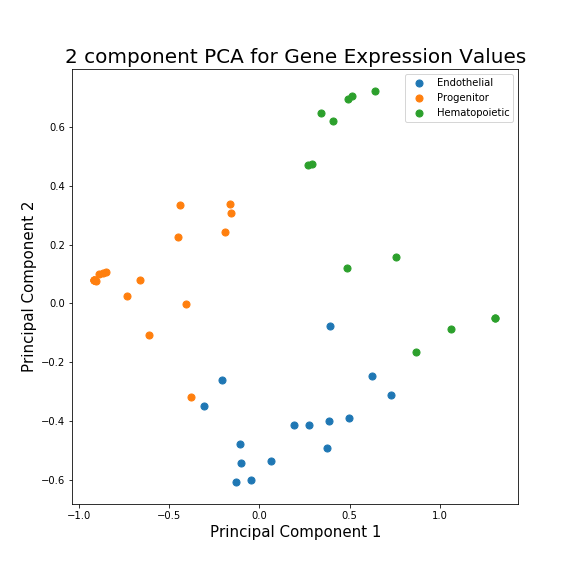
\includegraphics[height = 0.4\textheight]{../Preliminary/genepca.png}
		\caption{Genes represented after PCA transformation and grouped by unsupervised clustering into three clusters.}
		\label{fig:genePCA}
	\end{figure}
		We then plotted the actual mean expression values of the different genes grouped by their infered categories (see Fig). We clearly see the distinction in between groups, the clear expression of genes categorized as Hematopoietic in the 4SG stage as well as the expression of Endothelial genes in the 4SFG stage. 
	\begin{figure}[h!]
		\centering
		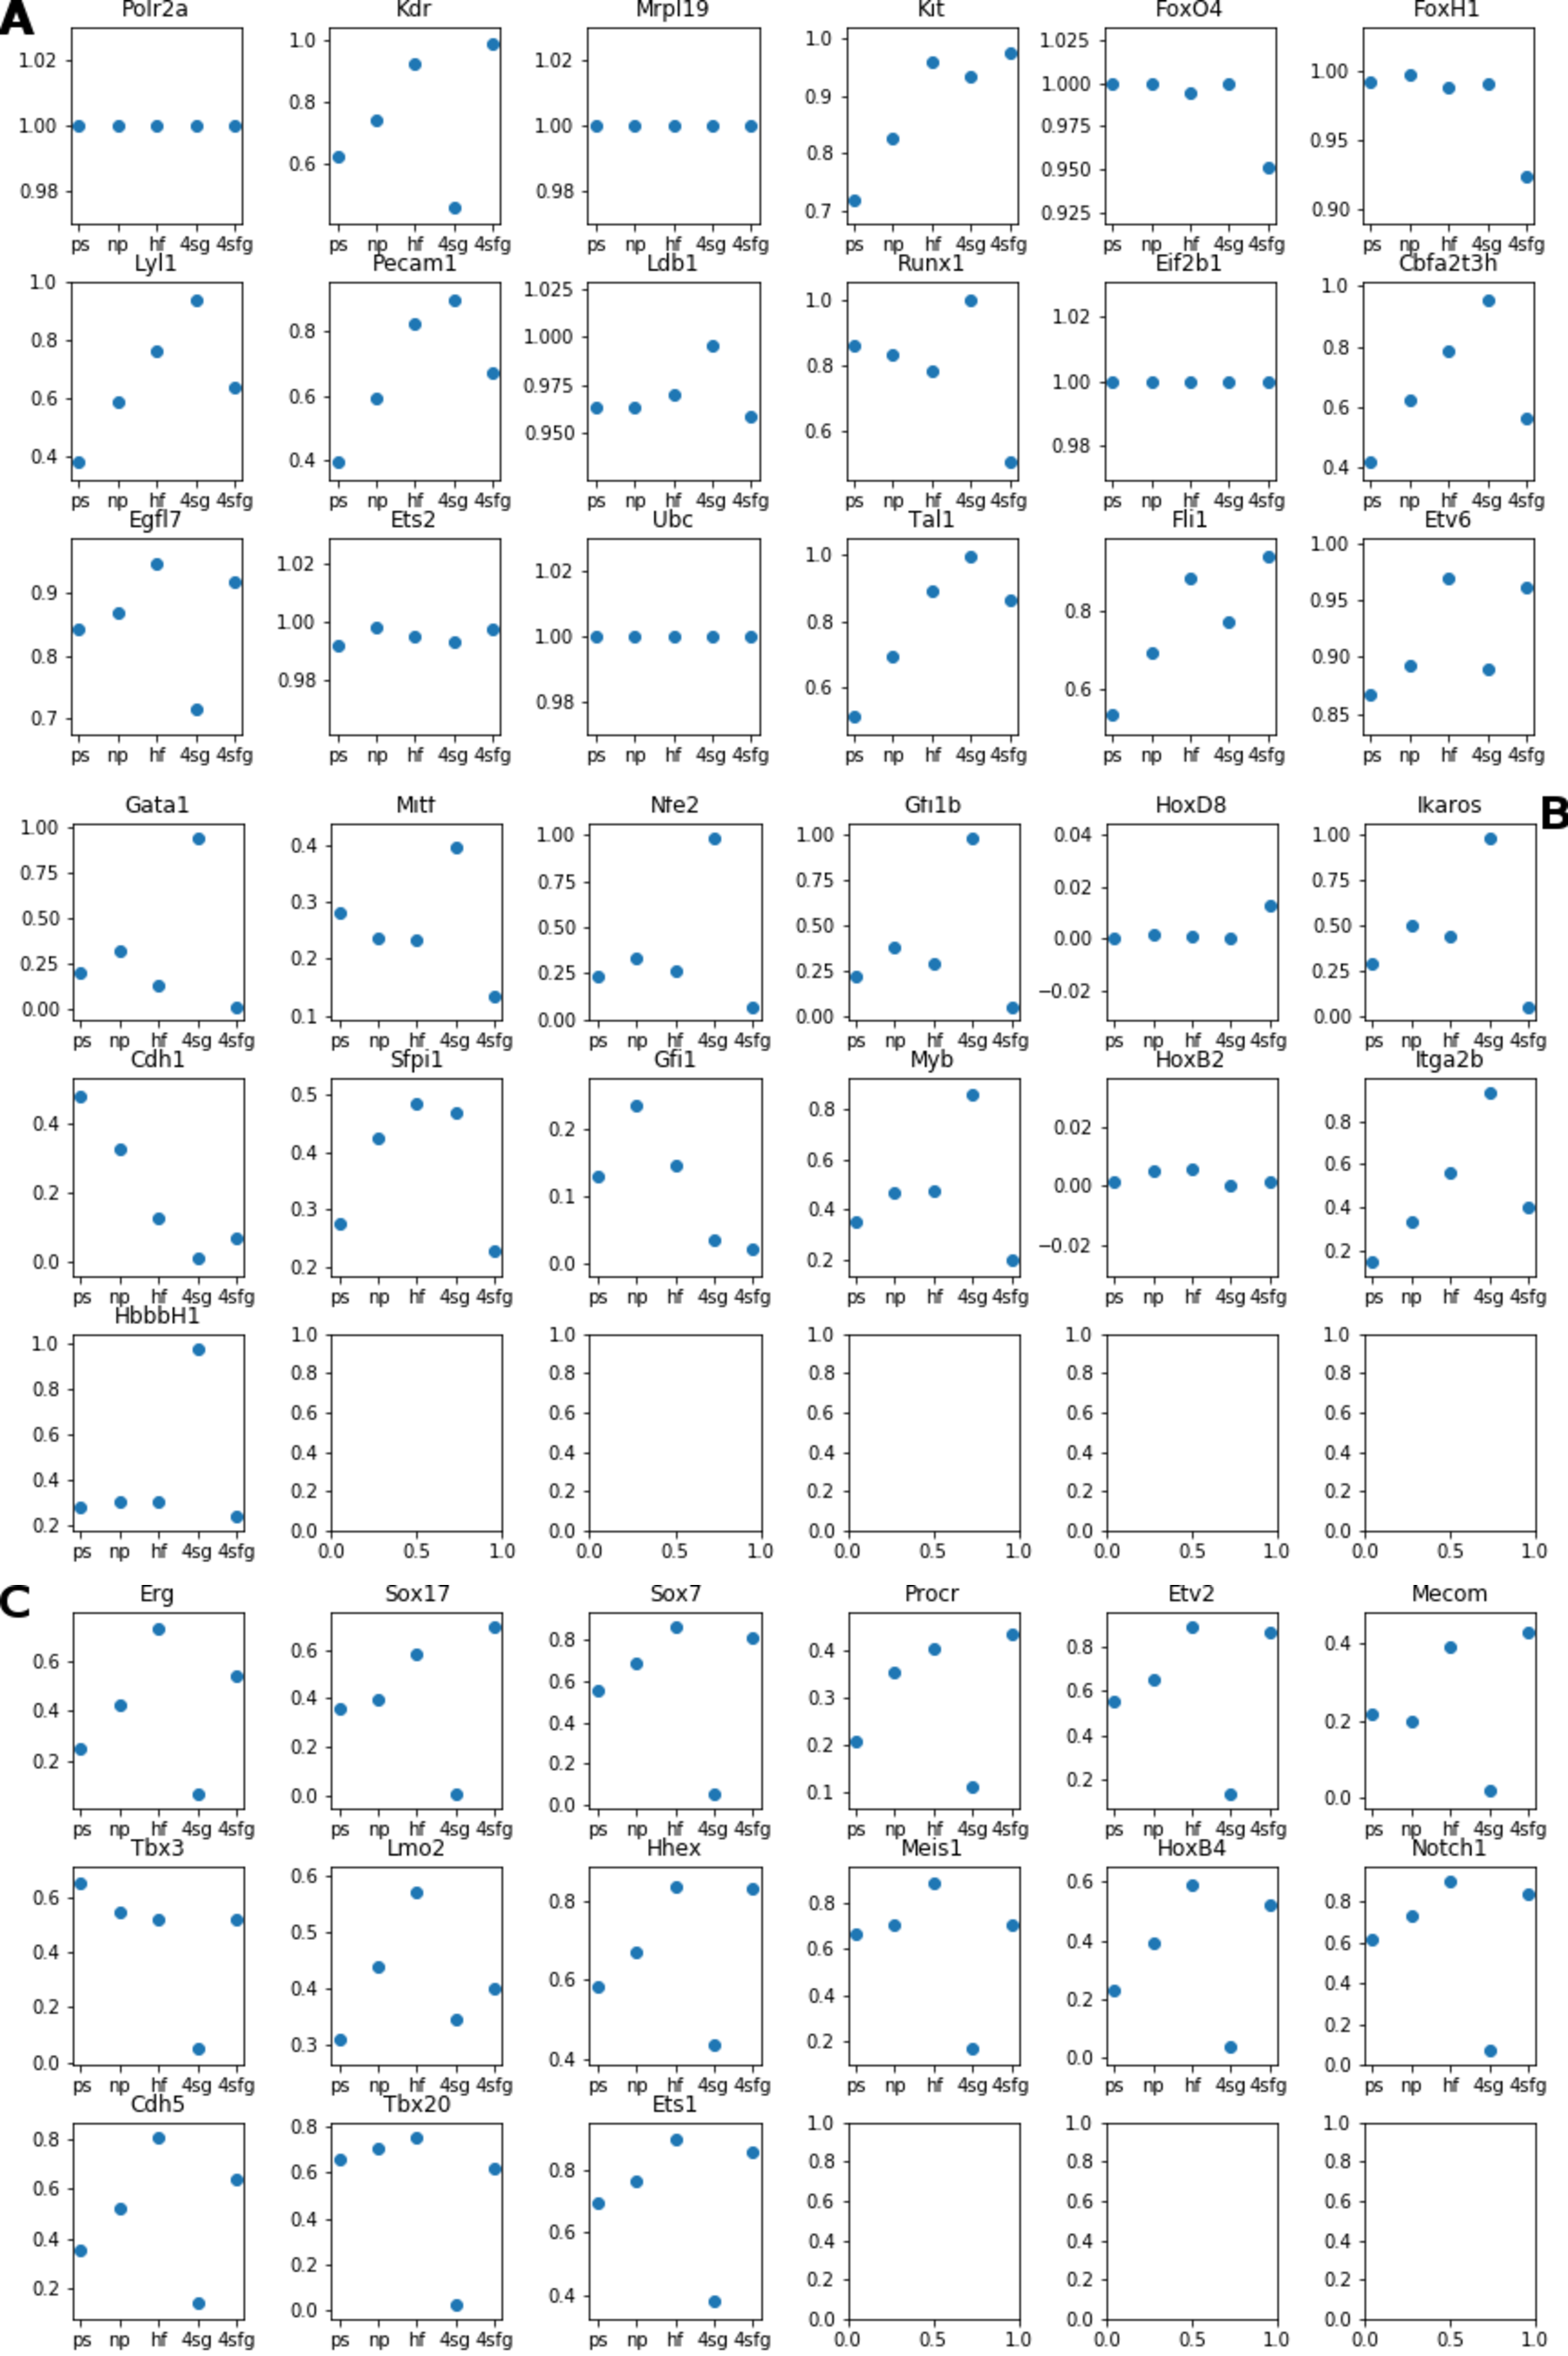
\includegraphics[width = 0.9\linewidth, height = 0.8\textheight]{../Preliminary/exptot.pdf}
		\caption{Mean gene expression values throughout the experiment. \textbf{A} Precursor genes \textbf{B} Hematopoietic genes \textbf{C} Endothelial genes}
		\label{fig:meangene}
	\end{figure}


\section*{Their Network Inference Method}
 The network inference tool used in the article was specially developed for their purpose. And indeed it achieves good results. Moreover it is explanatory, in the sense that it provides the update function of each gene as a boolean fucntion. We were first tempted to implement it but we finally decided, the amount of work was excessive. Still it is interesting to descibe their method.
 
 \paragraph{State-transition Graph}
 
 
\section*{Using MIIC}
	\begin{figure}[h!]
		\centering
		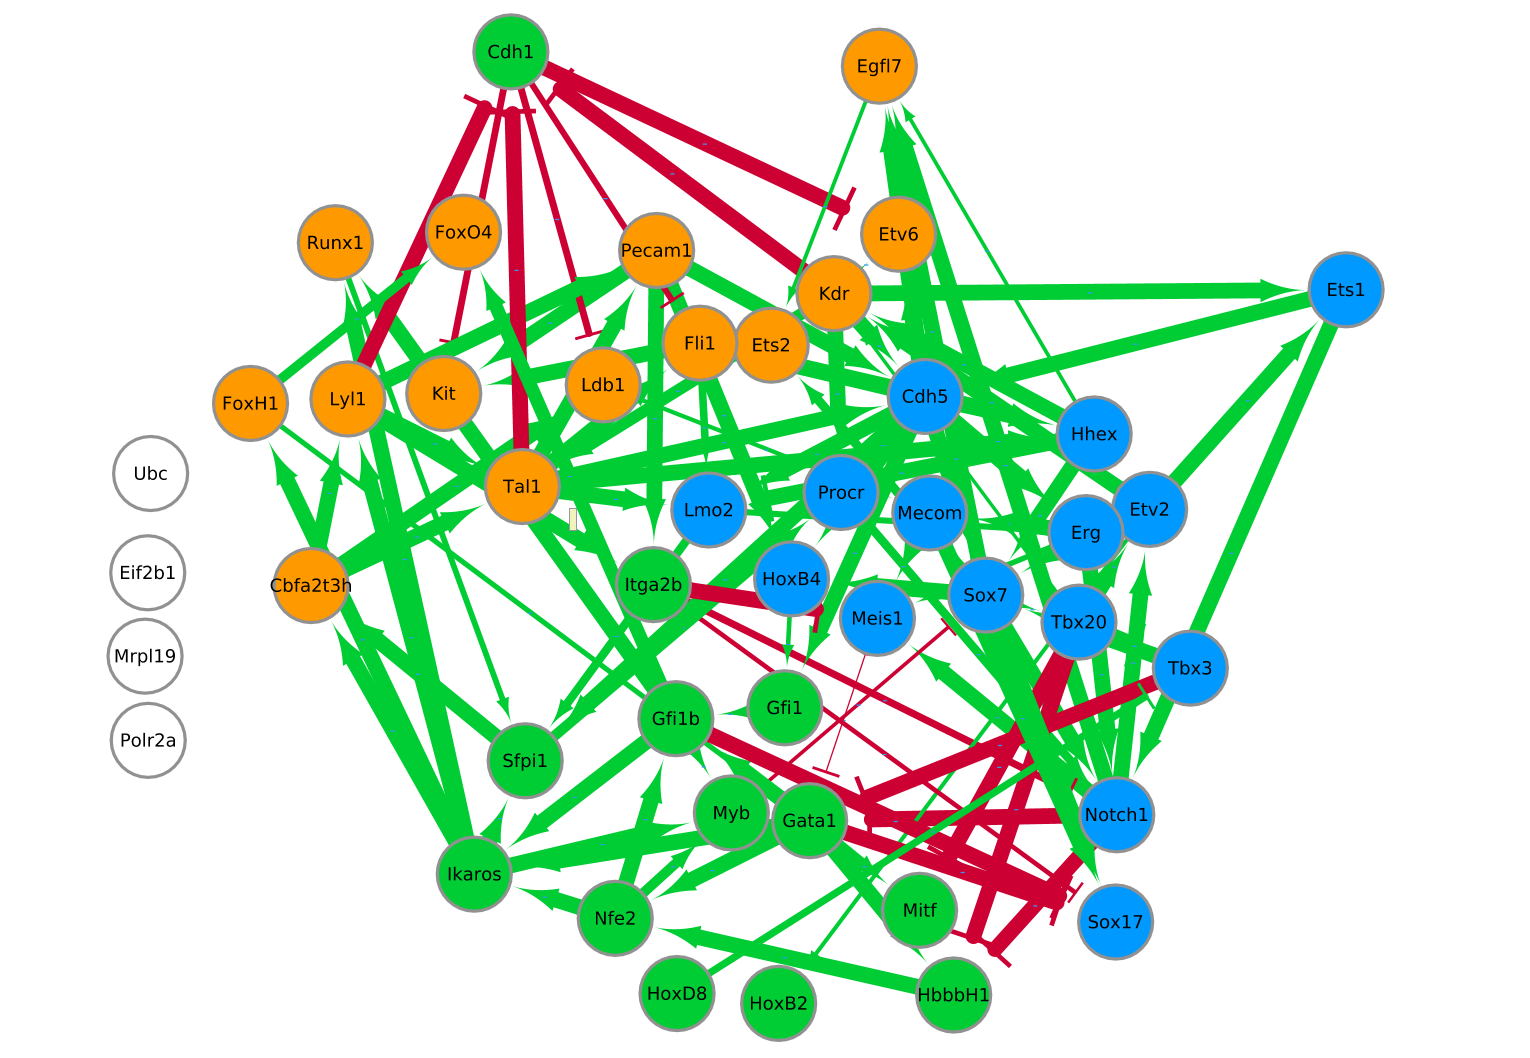
\includegraphics[width =\linewidth]{../MIIC-master/common/result/network.png}
		\caption{Network Inferred by MIIC. \textcolor{orange}{Precursor genes}, \textcolor{green}{ Hematopoietic genes} and  \textbf{C} Endothelial genes}
		\label{fig:miicnetwork}
	\end{figure}
\section*{Discussion}

	
\end{document}